\documentclass{article}
\usepackage[T1]{fontenc}
\usepackage{lmodern}
\usepackage{graphicx}
\usepackage{amsmath,amssymb}
\usepackage[a4paper,margin=2cm]{geometry}
\usepackage[absolute,overlay]{textpos}
\setlength{\TPHorizModule}{1mm}
\setlength{\TPVertModule}{1mm}
\usepackage[indonesian]{babel}
\usepackage{hyperref}
\setlength{\emergencystretch}{2em}
% unit: Halaman 14

\begin{document}

% === Halaman 14 (python/native) ===

Pliny the Elder menjelaskan penggunaan 

tinta dari getah tanaman thithymallus. Jika 

dituliskan pada kertas maka tulisan dengan 

tinta tersebut tidak kelihatan, tetapi bila 

kertas dipanaskan berubah menjadi 

gelap/coklat

Pliny the Elder. 

AD 23 - 79 

•  Penggunaan tinta tak-tampak (invisible ink)

14

% deskripsi: gambar native xref 103
\noindent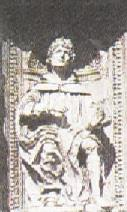
\includegraphics[width=0.85\textwidth]{../../images/python/page_014_img_01.jpeg}

\end{document}
